%%%%%%%%%%%%%%%%%%%%%%%%%%%%%%%%%%%%%%%%%
% Beamer Presentation
% LaTeX Template
% Version 2.0 (March 8, 2022)
%
% This template originates from:
% https://www.LaTeXTemplates.com
%
% Author:
% Vel (vel@latextemplates.com)
%
% License:
% CC BY-NC-SA 4.0 (https://creativecommons.org/licenses/by-nc-sa/4.0/)
%
%%%%%%%%%%%%%%%%%%%%%%%%%%%%%%%%%%%%%%%%%

%----------------------------------------------------------------------------------------
%	PACKAGES AND OTHER DOCUMENT CONFIGURATIONS
%----------------------------------------------------------------------------------------

\documentclass[
	8pt, % Set the default font size, options include: 8pt, 9pt, 10pt, 11pt, 12pt, 14pt, 17pt, 20pt
	%t, % Uncomment to vertically align all slide content to the top of the slide, rather than the default centered
	%aspectratio=169, % Uncomment to set the aspect ratio to a 16:9 ratio which matches the aspect ratio of 1080p and 4K screens and projectors
]{beamer}

\graphicspath{{Images/}{./}} % Specifies where to look for included images (trailing slash required)

\usepackage{booktabs} % Allows the use of \toprule, \midrule and \bottomrule for better rules in tables
\usepackage[font=footnotesize,labelfont=bf]{caption}
%----------------------------------------------------------------------------------------
%	SELECT LAYOUT THEME
%----------------------------------------------------------------------------------------

% Beamer comes with a number of default layout themes which change the colors and layouts of slides. Below is a list of all themes available, uncomment each in turn to see what they look like.

%\usetheme{default}
%\usetheme{AnnArbor}
%\usetheme{Antibes}
%\usetheme{Bergen}
%\usetheme{Berkeley}
%\usetheme{Berlin}
%\usetheme{Boadilla}
%\usetheme{CambridgeUS}
%\usetheme{Copenhagen}
%\usetheme{Darmstadt}
%\usetheme{Dresden}
%\usetheme{Frankfurt}
%\usetheme{Goettingen}
%\usetheme{Hannover}
%\usetheme{Ilmenau}
%\usetheme{JuanLesPins}
%\usetheme{Luebeck}
\usetheme{Madrid}
%\usetheme{Malmoe}
%\usetheme{Marburg}
%\usetheme{Montpellier}
%\usetheme{PaloAlto}
%\usetheme{Pittsburgh}
%\usetheme{Rochester}
%\usetheme{Singapore}
%\usetheme{Szeged}
%\usetheme{Warsaw}

%----------------------------------------------------------------------------------------
%	SELECT COLOR THEME
%----------------------------------------------------------------------------------------

% Beamer comes with a number of color themes that can be applied to any layout theme to change its colors. Uncomment each of these in turn to see how they change the colors of your selected layout theme.

%\usecolortheme{albatross}
%\usecolortheme{beaver}
%\usecolortheme{beetle}
%\usecolortheme{crane}
%\usecolortheme{dolphin}
%\usecolortheme{dove}
%\usecolortheme{fly}
%\usecolortheme{lily}
%\usecolortheme{monarca}
%\usecolortheme{seagull}
%\usecolortheme{seahorse}
%\usecolortheme{spruce}
%\usecolortheme{whale}
%\usecolortheme{wolverine}

%----------------------------------------------------------------------------------------
%	SELECT FONT THEME & FONTS
%----------------------------------------------------------------------------------------

% Beamer comes with several font themes to easily change the fonts used in various parts of the presentation. Review the comments beside each one to decide if you would like to use it. Note that additional options can be specified for several of these font themes, consult the beamer documentation for more information.

\usefonttheme{default} % Typeset using the default sans serif font
%\usefonttheme{serif} % Typeset using the default serif font (make sure a sans font isn't being set as the default font if you use this option!)
%\usefonttheme{structurebold} % Typeset important structure text (titles, headlines, footlines, sidebar, etc) in bold
%\usefonttheme{structureitalicserif} % Typeset important structure text (titles, headlines, footlines, sidebar, etc) in italic serif
%\usefonttheme{structuresmallcapsserif} % Typeset important structure text (titles, headlines, footlines, sidebar, etc) in small caps serif

%------------------------------------------------

%\usepackage{mathptmx} % Use the Times font for serif text
\usepackage{palatino} % Use the Palatino font for serif text

%\usepackage{helvet} % Use the Helvetica font for sans serif text
\usepackage[default]{opensans}
\usepackage{graphicx}
\usepackage{amsfonts}
\usepackage{wasysym}
\usepackage{csquotes} % Use the Open Sans font for sans serif text
%\usepackage[default]{FiraSans} % Use the Fira Sans font for sans serif text
%\usepackage[default]{lato} % Use the Lato font for sans serif text

\usepackage{bbm}
\usepackage{amsmath}
\usepackage{textcomp}
\usepackage{stmaryrd}

\usepackage{xcolor,colortbl}

%----------------------------------------------------------------------------------------
%	SELECT INNER THEME
%----------------------------------------------------------------------------------------

% Inner themes change the styling of internal slide elements, for example: bullet points, blocks, bibliography entries, title pages, theorems, etc. Uncomment each theme in turn to see what changes it makes to your presentation.

%\useinnertheme{default}
\useinnertheme{circles}
%\useinnertheme{rectangles}
%\useinnertheme{rounded}
%\useinnertheme{inmargin}

%----------------------------------------------------------------------------------------
%	SELECT OUTER THEME
%----------------------------------------------------------------------------------------

% Outer themes change the overall layout of slides, such as: header and footer lines, sidebars and slide titles. Uncomment each theme in turn to see what changes it makes to your presentation.

%\useoutertheme{default}
%\useoutertheme{infolines}
%\useoutertheme{miniframes}
%\useoutertheme{smoothbars}
%\useoutertheme{sidebar}
%\useoutertheme{split}
%\useoutertheme{shadow}
%\useoutertheme{tree}
%\useoutertheme{smoothtree}

%\setbeamertemplate{footline} % Uncomment this line to remove the footer line in all slides
%\setbeamertemplate{footline}[page number] % Uncomment this line to replace the footer line in all slides with a simple slide count

%\setbeamertemplate{navigation symbols}{} % Uncomment this line to remove the navigation symbols from the bottom of all slides

%----------------------------------------------------------------------------------------
%	PRESENTATION INFORMATION
%----------------------------------------------------------------------------------------

\title[Master's Thesis]{Gaussian Processes for the Analysis of Unequally Spaced Time Series} % The short title in the optional parameter appears at the bottom of every slide, the full title in the main parameter is only on the title page

%\subtitle{Optional Subtitle} % Presentation subtitle, remove this command if a subtitle isn't required

\author[Gianna Marano]{} % Presenter name(s), the optional parameter can contain a shortened version to appear on the bottom of every slide, while the main parameter will appear on the title slide

%\institute[UC]{University of Cambridge \\ \smallskip \textit{james@LaTeXTemplates.com}} % Your institution, the optional parameter can be used for the institution shorthand and will appear on the bottom of every slide after author names, while the required parameter is used on the title slide and can include your email address or additional information on separate lines
%
%\date[\today]{International Symposium of Explorers \\ \today} % Presentation date or conference/meeting name, the optional parameter can contain a shortened version to appear on the bottom of every slide, while the required parameter value is output to the title slide

%----------------------------------------------------------------------------------------

\begin{document}

%----------------------------------------------------------------------------------------
%	TITLE SLIDE
%----------------------------------------------------------------------------------------

\begin{frame}
	\titlepage % Output the title slide, automatically created using the text entered in the PRESENTATION INFORMATION block above
\end{frame}

%----------------------------------------------------------------------------------------
%	TABLE OF CONTENTS SLIDE
%----------------------------------------------------------------------------------------

% The table of contents outputs the sections and subsections that appear in your presentation, specified with the standard \section and \subsection commands. You may either display all sections and subsections on one slide with \tableofcontents, or display each section at a time on subsequent slides with \tableofcontents[pausesections]. The latter is useful if you want to step through each section and mention what you will discuss.

\begin{frame}
	\frametitle{Presentation Overview} % Slide title, remove this command for no title

	\tableofcontents % Output the table of contents (all sections on one slide)
	%\tableofcontents[pausesections] % Output the table of contents (break sections up across separate slides)
\end{frame}

%----------------------------------------------------------------------------------------
%	PRESENTATION BODY SLIDES
%----------------------------------------------------------------------------------------

\section{Objective and Problem Statement} % Sections are added in order to organize your presentation into discrete blocks, all sections and subsections are automatically output to the table of contents as an overview of the talk but NOT output in the presentation as separate slides

%------------------------------------------------

%\subsection{Bayesian Inference}\label{subsec:bayesian-inference}

\begin{frame}
	\frametitle{Problem Statement}

		\begin{figure}
				\includegraphics[width=0.8\linewidth]{new_measures_normy_plot_sind_rbf_seasonal_default_plot_true_with_samples.pdf}
				\caption{One week BP time series with unequally spaced samples. Sampling might not happen
				uniformly across time, e.g. more samples at day vs. night time}. Sampling frequency = 2/h
		\end{figure}

\end{frame}


\begin{frame}
	\frametitle{Problem Statement}

		Extracting Time Series characteristics (target measures) such as
		\begin{itemize}
		\item hourly/daily/weekly mean
		\item time in target range
		\item day and night blood pressure
		\end{itemize}

	\bigskip % Vertical whitespace

	Empirical averages are biased estimator of the hourly/daily/nightly/weekly mean if
	the samples are not uniformly distributed across time.

\end{frame}


\begin{frame}
	\frametitle{Objective}

		\begin{figure}
				\includegraphics[width=0.8\linewidth]{new_measures_normy_plot_mean_dec_sin_rbf_seasonal_default_plot_posterior_5}
				\caption{Black solid line: predicted mean. Gray area: predicted standard deviation}
		\end{figure}

	Ideally:
	\begin{itemize}
		\item unbiased estimates of the BP value as a function of time (from which all target
		measures can be extracted)
		\item uncertainty estimates, that can capture the uncertainty due to the lack of data
	\end{itemize}
\end{frame}



\section{Gaussian Process Regression} % Sections are added in order to organize your presentation into discrete blocks, all sections and subsections are automatically output to the table of contents as an overview of the talk but NOT output in the presentation as separate slides

%------------------------------------------------
\subsection{Introduction}

\begin{frame}
	\frametitle{Gaussian Process Regression}


	\textbf{Regression:} establish a mapping between the input variable $x$ and its corresponding output $f(x)$.
	\bigskip % Vertical whitespace

	In order to solve such a problem one usually needs some additional constraints on $f(x)$:

	\bigskip % Vertical whitespace
	\textbf{Parametric approach:} Restrict to a class of functions with parameters, e.g. linear functions. Parameters
	are inferred e.g through ML estimation (frequentist) or MAP estimation (bayesian).


	\bigskip % Vertical whitespace
	\textbf{Non-parametric and Bayesian regression:}
	Assign prior probabilities to all possible functions, giving higher probabilities to those considered more plausible.
	Inference revolves around the posterior distribution of these functions,
	given some potentially noisy observations of $f(x)$. If a Gaussian Process (GP) prior is used, we call it
	Gaussian Process regression.

\end{frame}


\begin{frame}
	\frametitle{Bayesian Inference}
	\begin{figure}
			\includegraphics[width=0.5\linewidth]{bayesian_learining}
			\caption{Bivariate Gaussian distribution. Joint (prior) distribution represented by ellipse. Black solid line
			represent the marginal (prior) marginal distributions p(x1), p(x2). Observing X1 changes our believe about
			X2, giving rise to the conditional (posterior) distribution (black dashed-dot line)}
	\end{figure}

\end{frame}


\subsection{Gaussian Process Definition}

\begin{frame}
	\frametitle{Gaussian Process Definition}


A Gaussian process (GP) can be viewed as a Gaussian distribution over functions or as an infinite set of random
variables representing the values of the function $f(x)$ at location $x$.
The Gaussian process is thus a generalization of the Gaussian distribution and a formal definition is given
by:

\begin{definition}[Gaussian Process]\label{def:GP}
 A Gaussian process is a collection of random variables, any finite number of which have a joint Gaussian distribution.
\end{definition}

\end{frame}


\begin{frame}
	\frametitle{Gaussian Process Definition}

As a (multivariate) Gaussian distribution is defined by its mean and covariance matrix, a GP is
uniquely identified by its mean $m(x)$ and covariance (kernel) function $k(x,x')$.

We write

\begin{gather*}
    f(x) \sim GP(m(x), k(x,x'))
\end{gather*}
with
\begin{gather*}
    m(x) = \mathbb{E}[f(x)] \\
    k(x,x') = \mathbb{E}[(f(x)-m(x))(f(x')-m(x'))]
\end{gather*}
\end{frame}


\begin{frame}
	\frametitle{Gaussian Process Samples}

	\begin{figure}
			\includegraphics[width=0.5\linewidth]{prior_samples}
			\caption{5 samples from a GP with $m(x)=0$  and $k(x,x') = \exp(-\frac{x-x'}{3}) +
			9 * \exp(-\frac{2 \sin^2(\frac{\pi |x -x'|}{24})}{9}) + \exp(-\frac{(x-x')^2}{2 * 30^2}) $}
	\end{figure}


\end{frame}


\begin{frame}
	\frametitle{Gaussian Process Definition}


If we assume $X$ to be the index set or set of possible inputs of $f$, then there is a random variable
$F_x := f(x)$ such that for a set $A \subset X$ with $A={x_1, \dots x_n}$ it holds that:

\[F_A = [F_{x_1}, \dots , F_{x_n}] \sim N(\mu_A,\,K_{AA})\]
for
\begin{gather}\label{def:Kernel-Matrix}
    K_{AA} =
    \begin{bmatrix}
        k(x_1, x_1) & k(x_1, x_2) & \dots & k(x_1, x_n)\\
        \vdots  &  & \vdots  & \vdots \\
        k(x_n, x_1)  & k(x_n, x_1) & \dots  & k(x_n, x_n)
    \end{bmatrix} \text{and }
    \mu_A =
    \begin{bmatrix}
        m(x_1) \\
        \vdots \\
        m(x_n)
    \end{bmatrix}
\end{gather}

The finite marginals $F_{x_1}, \dots, F_{x_n}$ of the GP thus have a multivariate gaussian distribution.
In our running example we might consider $X$ to be the time interval $T_0=[0, T]$ however it could be higher dimensional.

\end{frame}

\subsection{Gaussian Process Examples}

\begin{frame}
	\frametitle{Gaussian Process Examples}
	Note that a GP with finite index set and hence with joint Gaussian distribution is just a specific case
of GP. \\

	If we assume an ARMA process with gaussian innovations one can view the time series
as a collection of multivariate normally distributed random variables and thus as a GP.

	\[
        X_t =  \phi_1 X_{t-1} + \dots + \phi_p X_{t-p} + \theta_1 W_{t-1} + \dots \theta_q W_{t-q} + W_t
    \]
    where $W_t \stackrel{iid}{\sim} N(0, \sigma^2)$ is a gaussian white noise process.


\end{frame}


\subsection{Gaussian Process Inference}

\begin{frame}
	\frametitle{Predictive (Posterior Distribution)}

	General model for noisy blood pressure observations $Y(x)$ as a function of time $x \in \mathbb{R}$:

	\begin{align*}
		Y(x) = f(x) + \epsilon && \epsilon \sim N(0, \sigma_n^{2})
	\end{align*}

%	Assuming a linear model for $F_X = [f(x_1), \dots f(x_n)]^{\top}$ and:
%\begin{gather*}
%    F_X = X \beta + \mathbf{E}, \text{ with $\beta \sim N(0, \Sigma_p)$ and $\mathbf{E} \sim N(0, \Sigma_e)$}
%\end{gather*}

	\smallskip

	Prior distribution over the function $f(x)$:
	\begin{gather*}
		f(x) \sim GP(0, k(x, x')),
	\end{gather*}

	\smallskip

	\begin{figure}
			\includegraphics[width=0.4\linewidth]{bayesian_learining_mod}
			\caption{$f^{\ast} := f(x^\ast)$, the value we want to predict.
				$Y1 := Y(x1) = f(x1) + \epsilon$. $Y1 \sim N(0, k(x1,x1) + \sigma_n^2)$ and
				$f^{\ast} \sim N(0, k(x^{\ast}, x^{\ast}))$.
				We observe $y1$}
	\end{figure}

\end{frame}



\begin{frame}
	\frametitle{Bayesian Inference}
	\begin{figure}
			\includegraphics[width=0.4\linewidth]{bayesian_learining_mod}
			\caption{$f^{\ast} := f(x^\ast)$, the value we want to predict.
				$Y1 := Y(x1) = f(x1) + \epsilon$. We observe $y1$}
	\end{figure}

	The joint distribution (ellipse):
	\begin{gather}
		\begin{bmatrix}
			Y_1 \\
			f^{\ast}
		\end{bmatrix}
		\sim N \left(
			\begin{bmatrix}
			0 \\
			0
			\end{bmatrix},
			\begin{bmatrix}
			k(x_1, x_1) + \sigma_n^2 I & k(x_1, x^{\ast}) \\
			k(x^{\ast}, x_1) & k(x^{\ast}, x^{\ast})
			\end{bmatrix}
			\right)
		= p(Y_1, f^{\ast}| x_1, x^{\ast})
	\end{gather}

	The predictive distribution over $f^{\ast}$ (dashed-dot line):
	\begin{gather}
		p(f^{\ast}| Y_1 = y_1) = N(\bar{\mu}, \bar{\Sigma})
	\end{gather}

	where $\bar{\mu} = k(x^{\ast}, x_1) (k(x_1, x_1) + \sigma_n^2)^{-1} y_1$ \\
	and $\bar{\Sigma} = k(x^{\ast}, x^{\ast}) - k(x^{\ast}, x_1)(k(x_1, x_1) + \sigma_n^2)^{-1} k(x_1, x^{\ast})$

\end{frame}





\begin{frame}
	\frametitle{Bayesian Inference}

	 For a whole vector of observations $\mathbf{Y}$ and prediction time points $x^{\ast}$,
	 the joint distribution of $\mathbf{Y}$ and $f^{\ast} := f(x^{\ast})$ is given by:
	\begin{gather}
		\begin{bmatrix}
			\mathbf{Y} \\
			f^{\ast}
		\end{bmatrix}
		\sim N \left(
			\begin{bmatrix}
			0 \\
			0
			\end{bmatrix},
			\begin{bmatrix}
			K_{XX} + \sigma_n^2 I & K_{Xx^{\ast}} \\
			K_{x^{\ast}X} & K_{x^{\ast}x^{\ast}}
			\end{bmatrix}
			\right)
		= p(\mathbf{Y}, f^{\ast}| X, x^{\ast})
	\end{gather}


	The posterior (or predictive) distribution over $f^{\ast}$ can be derived by the well known conditioning rule for
		multivariate Gaussians:
	\begin{gather}
		p(f^{\ast}| \mathbf{Y}, X) = N(
	K_{x^{\ast}X} (K_{XX} + \sigma_n^2 I)^{-1} \mathbf{Y},
	K_{x^{\ast}x^{\ast}} - K_{x^{\ast}X}(K_{XX} + \sigma_n^2 I)^{-1}K_{Xx^{\ast}})
	\end{gather}

\end{frame}


\subsection{Kernel Functions}

\begin{frame}
	\frametitle{Kernel Functions}


	The kernel (or covariance) function $k(x,x')$ of a GP defines the dependency structure
	of the random variables $Y(x_1), \dots Y(x_n)$.
	\bigskip % Vertical whitespace

	It is equivalent to the concept of the autocovariance function in time series analysis:

	\begin{gather*}
    k(x, x') = \gamma_Y(x,x') = Cov(Y(x), Y(x')) = E[(Y(x) - \mu_Y(x))(Y(x')-\mu_Y(x'))]
	\end{gather*}

	\bigskip % Vertical whitespace


	Stationary kernels depend only on $\tau = x-x'$ and produce stationary time series (if mean function is constant)


\end{frame}

\begin{frame}
	\frametitle{Stationary Kernels - Squared Exponential}

	A.K.A. Radial Basis Function or Gaussian Kernel

	\begin{figure}
			\includegraphics[width=1\linewidth]{RBF_len}
			\caption{RBF kernel with different length scale}
	\end{figure}

	\begin{gather*}
    k(\tau) = \sigma^2 \exp(-\frac{\tau^2}{2 l^2})
	\end{gather*}
	with $l$ being the length scale and $\tau = x-x'$
\end{frame}

\begin{frame}
	\frametitle{Stationary Kernels - Matérn}


	\begin{figure}
			\includegraphics[width=1\linewidth]{Matern_3}
			\caption{Matérn Kernel with different $\nu$}
	\end{figure}

	Matern kernel
	\begin{gather*}
    k_{\nu}(\tau) = \sigma^2 \frac{2^{1-\nu}}{\Gamma(\nu)}(\frac{\sqrt{2\nu} \tau}{l})^{\nu} K_{\nu}
    (\frac{\sqrt{2\nu} \tau}{l})
	\end{gather*}

	when $\nu = \frac{1}{2}$ this is the continuous time analogue of an AR(1) process.

\end{frame}

\begin{frame}
	\frametitle{Stationary Kernels - Periodic Kernel}
	Periodic kernel: Expsinesquared kernel:

	\begin{figure}
			\includegraphics[width=1\linewidth]{sin_len}
			\caption{Periodic Kernel with different length scale}
	\end{figure}

	\begin{gather*}
    k(x, x') = \sigma^2 \exp(- \frac{2 \sin^2(\pi |x-x'| \backslash p)}{l^2})
	\end{gather*}

	where $p$ is the period
\end{frame}

\section{Methods}

\begin{frame}
	\frametitle{Methods}
	\framesubtitle{Overview}

	\begin{itemize}
		\item Simulate BP Time Series
	\end{itemize}

	\bigskip % Vertical whitespace

	\begin{itemize}
		\item For target measure compare performance of GP regression to baseline methods:
		\begin{itemize}
			\item Target measures: weekly daily and hourly mean, TTR
			\item Baseline Methods: Linear Regression, empirical overall mean, ttr naive, cubic spline
		\end{itemize}
	\end{itemize}

	\bigskip % Vertical whitespace

	\begin{itemize}
		\item Adversarial analysis: compare performance of baseline and GP regression introducing different adversarial
		factors
		\begin{itemize}
			\item Model mis-specification (mis-specified kernel or hyperparameters and non-gausianities)
			\item Missing data. More or less data available, more or less extreme non-uniform sampling patterns
		\end{itemize}

	\end{itemize}

\end{frame}

\subsection{BP Time Series Simulation}


\begin{frame}
	\frametitle{Methods - BP Time Series Simulation}
	\framesubtitle{Aktiia Population Level Time Series Characteristics - Part 1}

	Define GP such that its samples have similar characteristics:

	\begin{itemize}
		\item Within subject weekly BP sample variance $\approx 49 mmHg^2 = 7^2 mmHg^2$
			\begin{figure}
					\includegraphics[width=0.4\linewidth]{weekly_var}
					\caption{Distribution of weekly standard deviation within Aktiia population.
					Note: This is biased estimate of signal variance due to non-uniform sampling. In case
					of periodic sampling pattern, variance would be underestimated}
			\end{figure}
		\item measurement (Gaussian white) noise variance $=31 mmHg^2$
		\begin{itemize}
			\item Measured standard deviation of differences between SBP determinations of the Aktiia bracelet
			($BP_{Aktiia}$)  and double-auscultation ($BP_{Ref}$) = $7.92 mmHg$
			\item $Var(BP_{Ref} - BP_{Aktiia}) = 7.92^2 mmHg^2 = 62 mmHg^2 = Var(Noise_{Ref} - Noise_{Aktiia})
			= Var(Noise_{Ref}) + Var(Noise_{Aktiia}) - 2COV(Noise_{Ref}, Noise_{Aktiia})$
		\end{itemize}
	\end{itemize}
\end{frame}

\begin{frame}
	\frametitle{Methods - BP Time Series Simulation}
	\framesubtitle{Aktiia Population Level Time Series Characteristics - Part 2}

	Define GP such that its samples have similar characteristics:

	\begin{itemize}
		\item cyclic pattern amplitude $\approx 8 mmHg$
				\begin{figure}
					\includegraphics[width=0.3\linewidth]{20230531_LinTrap_amplitude_distrib}
					\caption{Aktiia night dip detection. ampl = $\frac{(\text{max-min})*2}{\pi}$}
				\end{figure}
		\begin{itemize}
			\item night dip amplitude (= avg night-avg day = $\frac{(\text{max-min})*2}{\pi}$) $ \approx 10 mmHg$
			\item cyclic pattern amplitude (=(max-min)/2) $\approx \frac{10 *\pi}{4} \approx 8 mmHg$
		\end{itemize}

	\end{itemize}

\end{frame}

\begin{frame}
	\frametitle{Methods - BP Time Series Simulation}
	\framesubtitle{Aktiia Population Level Time Series Characteristics - Part 3}

	Define GP such that its samples have similar characteristics:

	\begin{itemize}
		\item data density (0.5 to 4 per hour, i.e. 1.2 to 96 per day)
		\begin{figure}
			\includegraphics[width=0.4\linewidth]{20230531_number_of_valid_meas}
			\caption{Number of valid measurements}
		\end{figure}
		\item cyclic pattern period $= 24$ h
		\item AR(1) component with length scale 3 h and sample path variance $\approx 3.97 mmHg^2$
		\item long term trend variance $\approx 0.14 mmHg^2$
		\item cyclic data density pattern (e.g. less data during night, than during day and vice versa)
	\end{itemize}

\end{frame}

\begin{frame}[fragile]
	\frametitle{Methods - BP Time Series Simulation}
	\framesubtitle{GP Kernel Function}

	\begin{verbatim}

		Kernel = 2.24**2 * Matern(length_scale=3, nu=0.5)
				+ 14**2 * ExpSineSquared(length_scale=3, periodicity=24)
				+ 2.24**2 * RBF(length_scale=50)

	\end{verbatim}

	\begin{columns}[c] % The "c" option specifies centered vertical alignment while the "t" option is used for top vertical alignment
		\begin{column}{0.5\textwidth} % Left column width
				\begin{figure}
					\includegraphics[width=\linewidth]{new_measures_normy_plot_sin_rbf_default_plot_mean_decomposed_true}
					\caption{Decomposed posterior kernel function based on a sample drawn from
					a GP with additive kernel function}
				\end{figure}
		\end{column}
		\begin{column}{0.5\textwidth} % Right column width
				\begin{figure}
					\includegraphics[width=\linewidth]{new_measures_normy_plot_sin_rbf_default_plot_true_with_samples}
					\caption{True function f(x) (red dotted) with noisy measurements (red points)}
				\end{figure}

		\end{column}
	\end{columns}

\end{frame}

\begin{frame}
	\frametitle{Methods - BP Time Series Simulation}
	\framesubtitle{Comparison of Population Level Time Series Characteristics}
	300 draws from GP

			\begin{columns}[c] % The "c" option specifies centered vertical alignment while the "t" option is used for top vertical alignment
		\begin{column}{0.45\textwidth} % Left column width
				\begin{figure}
					\includegraphics[width=0.5\linewidth]{weekly_var}
					\caption{Aktiia Population Global SD}

				\end{figure}

			\begin{figure}
					\includegraphics[width=0.7\linewidth]{variance_y_true_std_summary}
					\caption{300 samples from GP Global SD}
			\end{figure}
		\end{column}
		\begin{column}{0.5\textwidth} % Right column width
				\begin{figure}
					\includegraphics[width=0.45\linewidth]{20230531_LinTrap_amplitude_distrib}
					\caption{Aktiia night dip detection. Night dip ampl=$\frac{(\text{max-min})*2}{\pi}$}
				\end{figure}

			\begin{figure}
					\includegraphics[width=0.6\linewidth]{variance_dip_ampl_summary}
					\caption{GP: 0.5 * night dip ampl $=\frac{\sqrt {2* \text{var(seasonal)}} * 2}{\pi}$)}
			\end{figure}


		\end{column}
	\end{columns}

\end{frame}


\subsection{Performance Evaluation}

\begin{frame}
	\frametitle{Methods}
	\framesubtitle{Overview}

	\begin{itemize}
		\item Simulate BP Time Series
	\end{itemize}

	\bigskip % Vertical whitespace

	\begin{itemize}
		\item For target measure compare performance of GP regression to baseline methods:
		\begin{itemize}
			\item Target measures: weekly daily and hourly mean, TTR
			\item Baseline Methods: Linear Regression, empirical overall mean, ttr naive, cubic spline
		\end{itemize}
	\end{itemize}

	\bigskip % Vertical whitespace

	\begin{itemize}
		\item Adversarial analysis: compare performance of baseline and GP regression introducing different adversarial
		factors
		\begin{itemize}
			\item Model mis-specification (mis-specified kernel or hyperparameters and non-gausianities)
			\item Missing data. More or less data available, more or less extreme non-uniform sampling patterns
		\end{itemize}

	\end{itemize}

\end{frame}


\begin{frame}
	\frametitle{Methods - Performance Evaluation}
	\framesubtitle{Simulation and Evaluation Flow}
		for i in $1 \dots n_{simulations}$:
		\begin{enumerate}
			\item Simulate from true GP (adversarial add non-Gaussian noise)
			\item Subsample data (adversarial: different densities, non-uniform sampling)
			\item Fit Regression
			\begin{itemize}
				\item Fit GP-Regression model (adversarial: prior covariance function diverges from true)
				\item Fit Baseline Method
			\end{itemize}
			\item Extract target measure including its distribution.
				\begin{itemize}
					\item GP: sample from the posterior distribution (Multivariate Gaussian) to approx. it.
					\item Baseline Methods: Use bootstrap to approx. it
				\end{itemize}
			\item Calculate performance metric between true and predicted values.
		\end{enumerate}

	\bigskip
	Calculate mean performance over $n_{simulations}$
		\begin{itemize}
			\item CI coverage of true value and CI width
		\end{itemize}

	\bigskip

	Compare performance of GP Regression to baseline methods

\end{frame}
%
%\begin{frame}
%	\frametitle{Methods - Performance Evaluation}
%	\framesubtitle{Simulation and GP Regression Details}
%	Simulation of true BP signal and measurements:
%		\begin{itemize}
%			\item $X=\{x_1, \dots x_n\}$: The input time points of interest, i.e. 1 week with 10 BP values per hour.
%			\item $f_X := \{f(x_1) \dots f(x_n)\}$: The true BP signal $f(x)$ drawn from $GP(0, k_{true}(x,x'))$ evaluated at inputs $X$.
%			\item $y_X := \{y(x_1) \dots y(x_n)\}$: The noisy BP measurements. $y(x)= f(x) + \epsilon$ with $\epsilon \sim N(0, \sigma_n^2)$
%		\end{itemize}
%	\bigskip
%	Based on subsampling scheme choose $X_{train} \subset X$ with $|X_{train}| = m$ and $X_{test} = X \setminus X_{train}$.
%	\begin{itemize}
%		\item $y_{train} := \{y(x_i) | x_i \in X_{train}\}$
%		\item  $f_{train} := \{f(x_i) | x_i \in X_{train}\}$
%	\end{itemize}
%
%	\bigskip
%
%	Fit GP regression model to training data $y_{train}$, $X_{train}$:
%			\begin{itemize}
%				\item $k_{fit}$: The fitted kernel function with hyperparameters $\theta$ that maximizes the marginal likelihood
%				$p(y_{train}| \theta)$
%				\item $p(f_X| y_{train}, k_{fit}) = N(\bar{\mu}, \bar{\Sigma})$:
%				The posterior (predictive) probability density of $f_X$. The posterior mean vector
%				$\bar{\mu} \in \mathbb{R}^n$ contains the point estimates for $f_X$.
%				\begin{itemize}
%					\item $\bar{\mu}_{train} := \{\bar{\mu}_i | x_i \in X_{train}\}$
%					\item $\bar{\Sigma}_{train} := \bar{\Sigma}_{i,j}$ where $\{i | x_i \in X_{train}\}$ and $\{j | x_j \in X_{train}\}$
%
%				\end{itemize}
%			\end{itemize}
%	\bigskip
%	Output of GP Regression are predictive probabilities $p(f_{train}| y_{train})$,
%		$p(f_{test}| y_{train})$ and $p(f_{X}| y_{train})$:
%			\begin{itemize}
%				\item Note $\bar{\mu}_{train} \neq f_{train}$ due to the measurement error. \\ If
%				$f_{train}$ was known: $p(f_{train}| f_{train}, GP_{fit}) = N(\bar{\mu}_{X_{train}},
%				\bar{\Sigma}_{X_{train}})$
%				with $\bar{\mu}_{train} = f_{train}$ and $\bar{\Sigma}_{train} = {\displaystyle O}$
%			\end{itemize}
%
%\end{frame}


\subsection{Baseline Methods}

\begin{frame}
	\frametitle{Methods - Baseline Methods}
	\framesubtitle{Overall mean}

		\begin{figure}
			\includegraphics[width=0.6\linewidth]{new_measures_normy_mean_dec_plot_sin_rbf_default_plot_posterior_overall_mean_9}
			\caption{1 week BP time series with 2 samples per hour (uniformly sampleed across time)}
		\end{figure}

\end{frame}

%\begin{frame}
%	\frametitle{Methods - Baseline Methods}
%	\framesubtitle{Naive TTR}
%		\begin{figure}
%			\includegraphics[width=0.6\linewidth]{new_measures_transform_qunatile_sin_rbf_default_08_19_14_50_32_plot_posterior_naive_ttr}
%			\caption{1 week BP time series with 2 samples per hour (uniformly sampleed across time)}
%		\end{figure}
%
%\end{frame}

\begin{frame}
	\frametitle{Methods - Baseline Methods}
	\framesubtitle{Linear Regression}
		\begin{figure}
			\includegraphics[width=0.6\linewidth]{new_measures_normy_mean_dec_plot_sin_rbf_default_plot_posterior_linear_9}
			\caption{1 week BP time series with 2 samples per hour (uniformly sampleed across time)}
		\end{figure}

	\begin{itemize}
		\item $Y(t) = \beta_0 + \beta_1 t + \beta_2 \cos(2 \pi f t) + \beta_3 \sin(2 \pi f t) + \epsilon, \epsilon \text{ iid } \sim N(0, \sigma^2)$
	\end{itemize}

\end{frame}

\begin{frame}
	\frametitle{Methods - Baseline Methods}
	\framesubtitle{Spline}
		\begin{figure}
			\includegraphics[width=0.6\linewidth]{new_measures_normy_mean_dec_plot_sin_rbf_default_plot_posterior_spline_9}
			\caption{1 week BP time series with 2 samples per hour (uniformly sampled across time)}
		\end{figure}

	\begin{itemize}
		\item smoothing parameter identified using cross validation
	\end{itemize}

\end{frame}

\subsection{Target Measures}

\begin{frame}
	\frametitle{Methods - Target Measures}

	Hourly/Daily/Weekly Mean
	\begin{itemize}
		\item Calculation:
		\begin{itemize}
			\item General: Mean of predicted values within the time period
			\item Naive TTR: Mean of available measurements within the time period. If no available measurement
			global mean is used
		\end{itemize}
	\end{itemize}

	\bigskip

	Time in Target Range (TTR):
	\begin{itemize}
		\item Target Range: 90 to 125 mmHg
		\item Calculation:
		\begin{itemize}
			\item General: Number of predicted data points within the range over the total number of data points
			\item Naive TTR: Number of available data points within the range over the total number of available data points
		\end{itemize}
	\end{itemize}

%	Calculate TTR:
%	\begin{itemize}
%			\item General: Number of predicted data points within the range over the total number of data points
%			\item Naive TTR: Number of available data points within the range over the total number of available data points
%			\item True: $\sum_{i=1}^{n} \mathbbm{1}\{\ f(x_i) < \gamma \}$.
%			\item GP/Spline/: $\sum_{i=1}^{n} \mathbbm{1}\{\ \bar{\mu}_i < \gamma \}$. Sample from Posterior to get CI
%			\item Naive: $\sum_{i=1, y_i \in y_{train}}^{m} \mathbbm{1}\{\ y_i < \gamma \}$
%	\end{itemize}

\end{frame}


%\subsection{Adversarial Analysis}
%
%\begin{frame}
%	\frametitle{Methods - Adversarial Analysis}
%
%	\begin{itemize}
%		\item Data density (0.5 to 4 mearurments per hour)
%		\item Seasonal sampling
%	\end{itemize}
%
%
%	\begin{figure}
%		\includegraphics[width=0.5\linewidth]{new_measures_transform_quantile_sin_rbf_seasonal_default_08_19_18_22_59_plot_true_with_samples.pdf}
%		\caption{Seasonal sampling with 2 samples per hour}
%	\end{figure}
%\end{frame}



\section{Results}

\begin{frame}
	\frametitle{Results - GP Regression}
	\framesubtitle{Uniform Sampling Example 1}

	GP fitted to 1 week BP time series with 2 samples per hour (uniformly sampled across time)

	\begin{columns}[c] % The "c" option specifies centered vertical alignment while the "t" option is used for top vertical alignment
		\begin{column}{0.5\textwidth} % Left column width
				\begin{figure}
					\includegraphics[width=\linewidth]{new_measures_normy_mean_dec_plot_sin_rbf_default_plot_posterior_9}
					\caption{Predictive Distribution. True function (red dashed line) with 2 samples (red dots) per hour}
				\end{figure}
		\end{column}
		\begin{column}{0.5\textwidth} % Right column width
				\begin{figure}
					\includegraphics[width=0.8\linewidth]{new_measures_normy_mean_dec_plot_sin_rbf_default_plot_mean_decomposed_9.pdf}
					\caption{True (upper figure) and predicted (lower figure) decomposed mean}
				\end{figure}

		\end{column}
	\end{columns}

\end{frame}



\begin{frame}
	\frametitle{Results - GP Regression vs Baseline}
	\framesubtitle{Uniform Sampling Example 1}

	\begin{columns}[c] % The "c" option specifies centered vertical alignment while the "t" option is used for top vertical alignment
		\begin{column}{0.5\textwidth} % Left column width
				\begin{figure}
					\includegraphics[width=\linewidth]{new_measures_normy_mean_dec_plot_sin_rbf_default_plot_posterior_9}
					\caption{Predictive Distribution. True function (red dashed line) with 2 samples (red dots) per hour}
				\end{figure}
		\end{column}
		\begin{column}{0.5\textwidth} % Right column width
				\begin{figure}
					\includegraphics[width=0.8\linewidth]{new_measures_normy_mean_dec_plot_sin_rbf_default_plot_posterior_linear_9}
					\caption{Linear}
				\end{figure}

				\begin{figure}
					\includegraphics[width=0.8\linewidth]{new_measures_normy_mean_dec_plot_sin_rbf_default_plot_posterior_spline_9}
					\caption{Spline}
				\end{figure}
		\end{column}
	\end{columns}

\end{frame}


\begin{frame}
	\frametitle{Results - GP Regression}
	\framesubtitle{Uniform Sampling Example 2}

	GP fitted to 1 week BP time series with 2 samples per hour (uniformly sampled across time)

	\begin{columns}[c] % The "c" option specifies centered vertical alignment while the "t" option is used for top vertical alignment
		\begin{column}{0.5\textwidth} % Left column width
				\begin{figure}
					\includegraphics[width=\linewidth]{new_measures_normy_mean_dec_plot_sin_rbf_default_plot_posterior_2}
					\caption{Predictive Distribution. True function (red dashed line) with 2 samples (red dots) per hour}
				\end{figure}
		\end{column}
		\begin{column}{0.5\textwidth} % Right column width
				\begin{figure}
					\includegraphics[width=0.8\linewidth]{new_measures_normy_mean_dec_plot_sin_rbf_default_plot_mean_decomposed_2}
					\caption{True (upper figure) and predicted (lower figure) decomposed mean}
				\end{figure}

		\end{column}
	\end{columns}

\end{frame}



\begin{frame}
	\frametitle{Results - GP Regression vs Baseline}
	\framesubtitle{Uniform Sampling Example 2}

	\begin{columns}[c] % The "c" option specifies centered vertical alignment while the "t" option is used for top vertical alignment
		\begin{column}{0.5\textwidth} % Left column width
				\begin{figure}
					\includegraphics[width=\linewidth]{new_measures_normy_mean_dec_plot_sin_rbf_default_plot_posterior_2}
					\caption{Predictive Distribution. True function (red dashed line) with 2 samples (red dots) per hour}
				\end{figure}
		\end{column}
		\begin{column}{0.5\textwidth} % Right column width
				\begin{figure}
					\includegraphics[width=0.8\linewidth]{new_measures_normy_mean_dec_plot_sin_rbf_default_plot_posterior_linear_2}
					\caption{Linear}
				\end{figure}

				\begin{figure}
					\includegraphics[width=0.8\linewidth]{new_measures_normy_mean_dec_plot_sin_rbf_default_plot_posterior_spline_2}
					\caption{Spline}
				\end{figure}
		\end{column}
	\end{columns}

\end{frame}


\begin{frame}
	\frametitle{Results - GP Regression}
	\framesubtitle{Seasonal Sampling Example  1}

	GP fitted to 1 week BP time series with 2 samples per hour (seasonal sampling)

		\begin{columns}[c] % The "c" option specifies centered vertical alignment while the "t" option is used for top vertical alignment
		\begin{column}{0.5\textwidth} % Left column width
				\begin{figure}
					\includegraphics[width=\linewidth]{new_measures_normy_plot_mean_dec_sin_rbf_seasonal_default_plot_posterior_5}
					\caption{Predictive Distribution. True function (red dashed line) with 2 samples (red dots) per hour}
				\end{figure}
		\end{column}
		\begin{column}{0.5\textwidth} % Right column width
				\begin{figure}
					\includegraphics[width=0.8\linewidth]{new_measures_normy_plot_mean_dec_sin_rbf_seasonal_default_plot_mean_decomposed_5}
					\caption{True (upper figure) and predicted (lower figure) decomposed mean}
				\end{figure}

		\end{column}
	\end{columns}

\end{frame}

\begin{frame}
	\frametitle{Results - GP Regression vs Baseline}
	\framesubtitle{Seasonal Sampling Example 1}

	\begin{columns}[c] % The "c" option specifies centered vertical alignment while the "t" option is used for top vertical alignment
		\begin{column}{0.5\textwidth} % Left column width
				\begin{figure}
					\includegraphics[width=\linewidth]{new_measures_normy_plot_mean_dec_sin_rbf_seasonal_default_plot_posterior_5}
					\caption{Predictive Distribution. True function (red dashed line) with 2 samples (red dots) per hour}
				\end{figure}
		\end{column}
		\begin{column}{0.5\textwidth} % Right column width
				\begin{figure}
					\includegraphics[width=0.8\linewidth]{new_measures_normy_plot_mean_dec_sin_rbf_seasonal_default_plot_posterior_linear_5}
					\caption{Linear}
				\end{figure}

				\begin{figure}
					\includegraphics[width=0.8\linewidth]{new_measures_normy_plot_mean_dec_sin_rbf_seasonal_default_plot_posterior_spline_5}
					\caption{Spline}
				\end{figure}
		\end{column}
	\end{columns}

\end{frame}




\begin{frame}
	\frametitle{Results - GP Regression}
	\framesubtitle{Seasonal Sampling Example  2}

	GP fitted to 1 week BP time series with 2 samples per hour (seasonal sampling)

		\begin{columns}[c] % The "c" option specifies centered vertical alignment while the "t" option is used for top vertical alignment
		\begin{column}{0.5\textwidth} % Left column width
				\begin{figure}
					\includegraphics[width=\linewidth]{new_measures_normy_plot_mean_dec_sin_rbf_seasonal_default_plot_posterior_9}
					\caption{Predictive Distribution. True function (red dashed line) with 2 samples (red dots) per hour}
				\end{figure}
		\end{column}
		\begin{column}{0.5\textwidth} % Right column width
				\begin{figure}
					\includegraphics[width=0.8\linewidth]{new_measures_normy_plot_mean_dec_sin_rbf_seasonal_default_plot_mean_decomposed_9}
					\caption{True (upper figure) and predicted (lower figure) decomposed mean}
				\end{figure}

		\end{column}
	\end{columns}

\end{frame}

\begin{frame}
	\frametitle{Results - GP Regression vs Baseline}
	\framesubtitle{Seasonal Sampling Example 2}

	\begin{columns}[c] % The "c" option specifies centered vertical alignment while the "t" option is used for top vertical alignment
		\begin{column}{0.5\textwidth} % Left column width
				\begin{figure}
					\includegraphics[width=\linewidth]{new_measures_normy_plot_mean_dec_sin_rbf_seasonal_default_plot_posterior_9}
					\caption{Predictive Distribution. True function (red dashed line) with 2 samples (red dots) per hour}
				\end{figure}
		\end{column}
		\begin{column}{0.5\textwidth} % Right column width
				\begin{figure}
					\includegraphics[width=0.8\linewidth]{new_measures_normy_plot_mean_dec_sin_rbf_seasonal_default_plot_posterior_linear_9}
					\caption{Linear}
				\end{figure}

				\begin{figure}
					\includegraphics[width=0.8\linewidth]{new_measures_normy_plot_mean_dec_sin_rbf_seasonal_default_plot_posterior_spline_9}
					\caption{Spline}
				\end{figure}
		\end{column}
	\end{columns}

\end{frame}

\begin{frame}
	\frametitle{Results}
	\framesubtitle{Weekly Mean} % Optional subtitle

	Simulation over a 100 samples from true GP

	\begin{figure}
			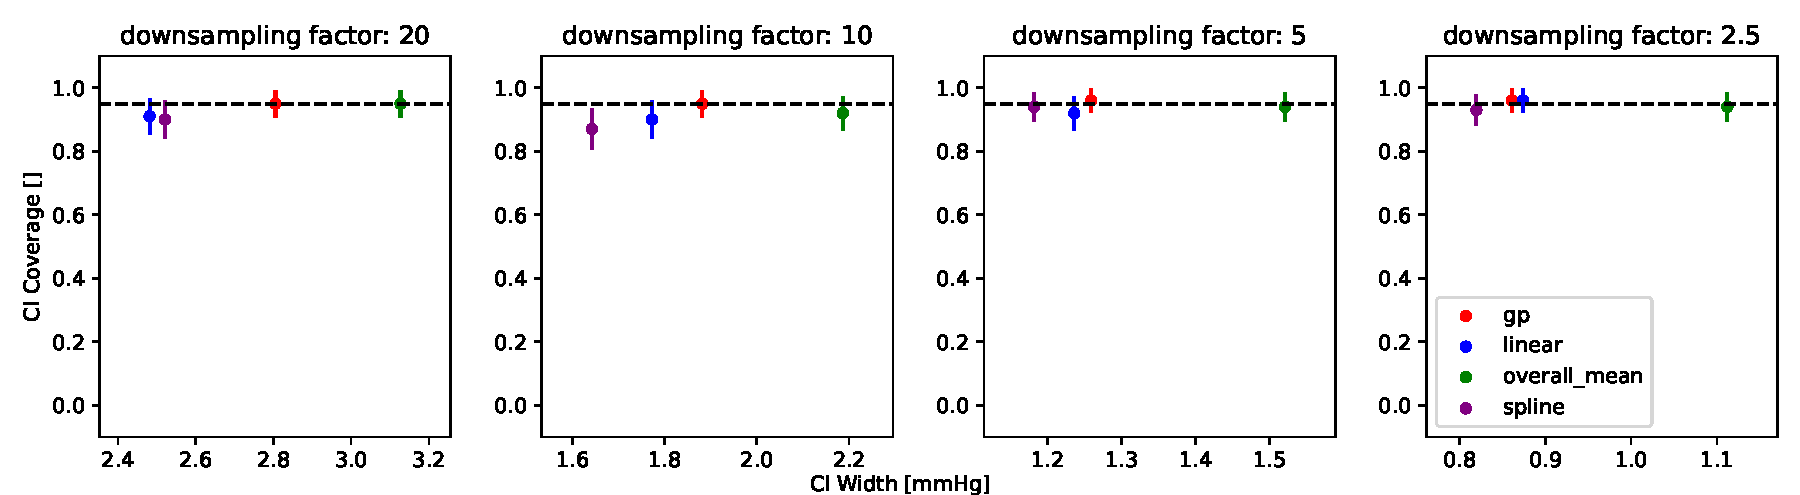
\includegraphics[width=0.8\linewidth]{overall_mean_eval_sin_rbf_default}
			\caption{Uniform Sampling}
	\end{figure}

	\begin{figure}
			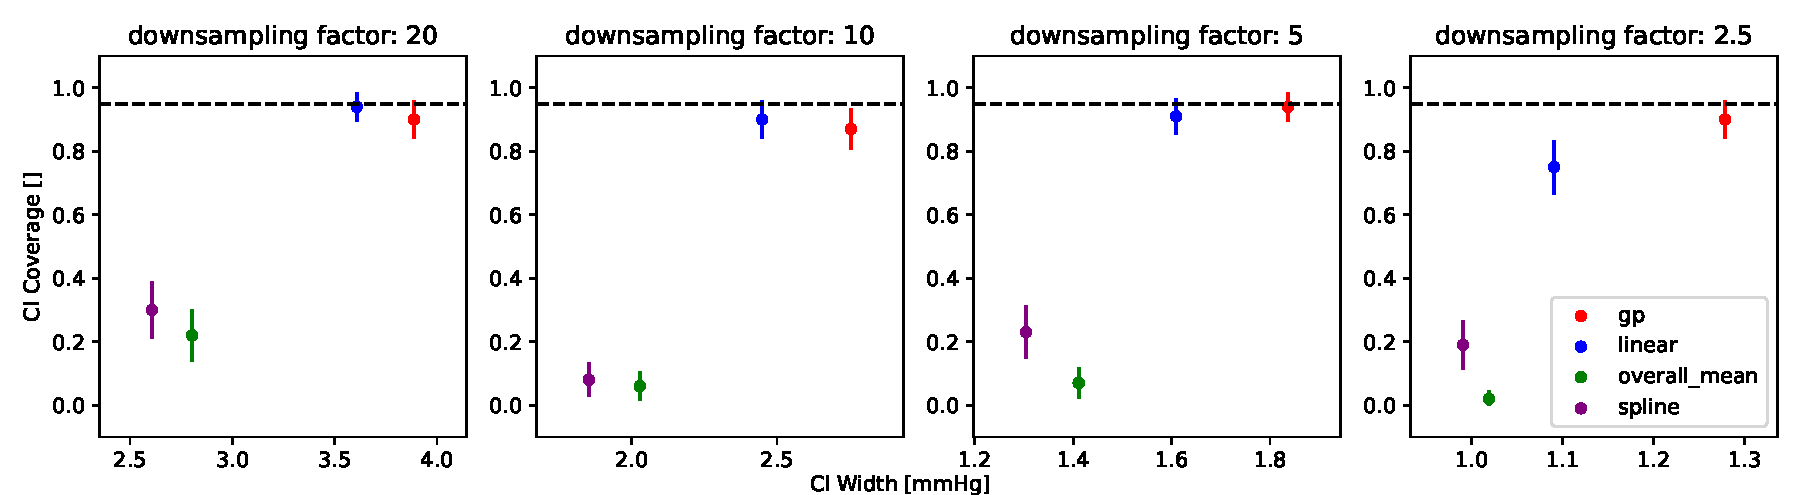
\includegraphics[width=0.8\linewidth]{overall_mean_eval_sin_rbf_seasonal_default}
			\caption{Seasonal Sampling}
	\end{figure}

\end{frame}


\begin{frame}
	\frametitle{Results}
	\framesubtitle{Hourly Mean} % Optional subtitle

	Simulation over a 100 samples from true GP

	\begin{figure}
			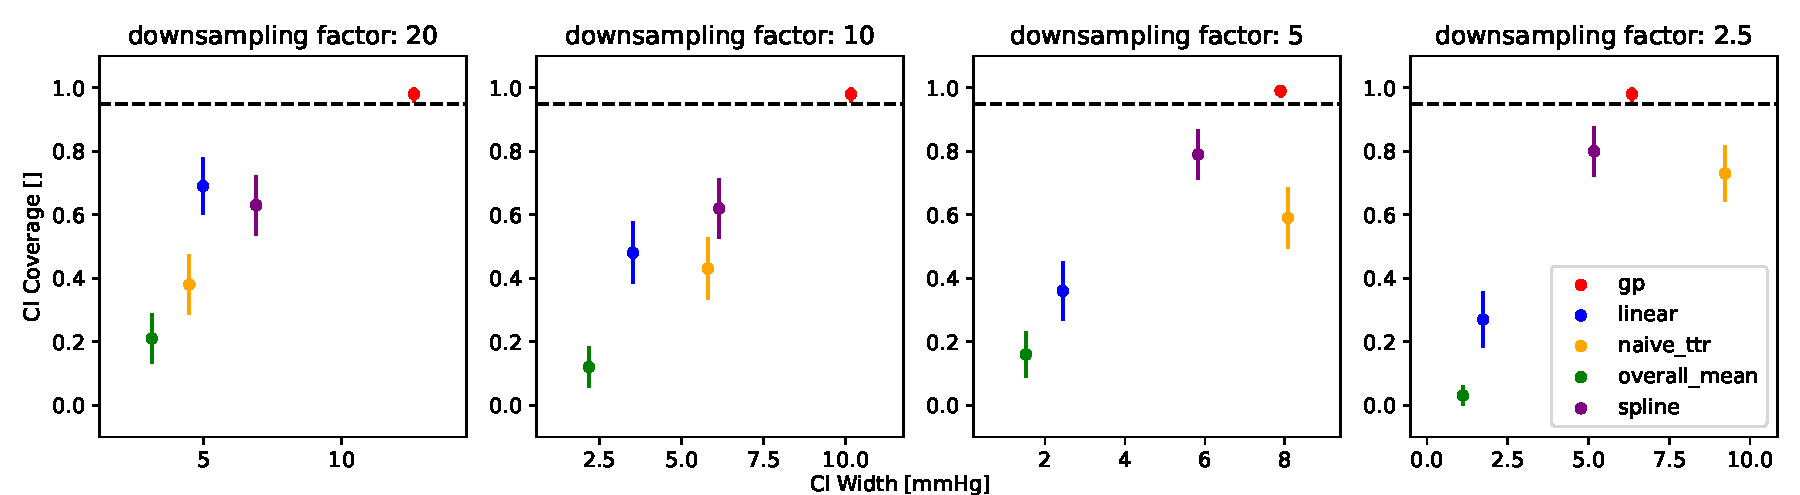
\includegraphics[width=0.8\linewidth]{mean_1h_eval_sin_rbf_default}
			\caption{Uniform Sampling}
	\end{figure}

	\begin{figure}
			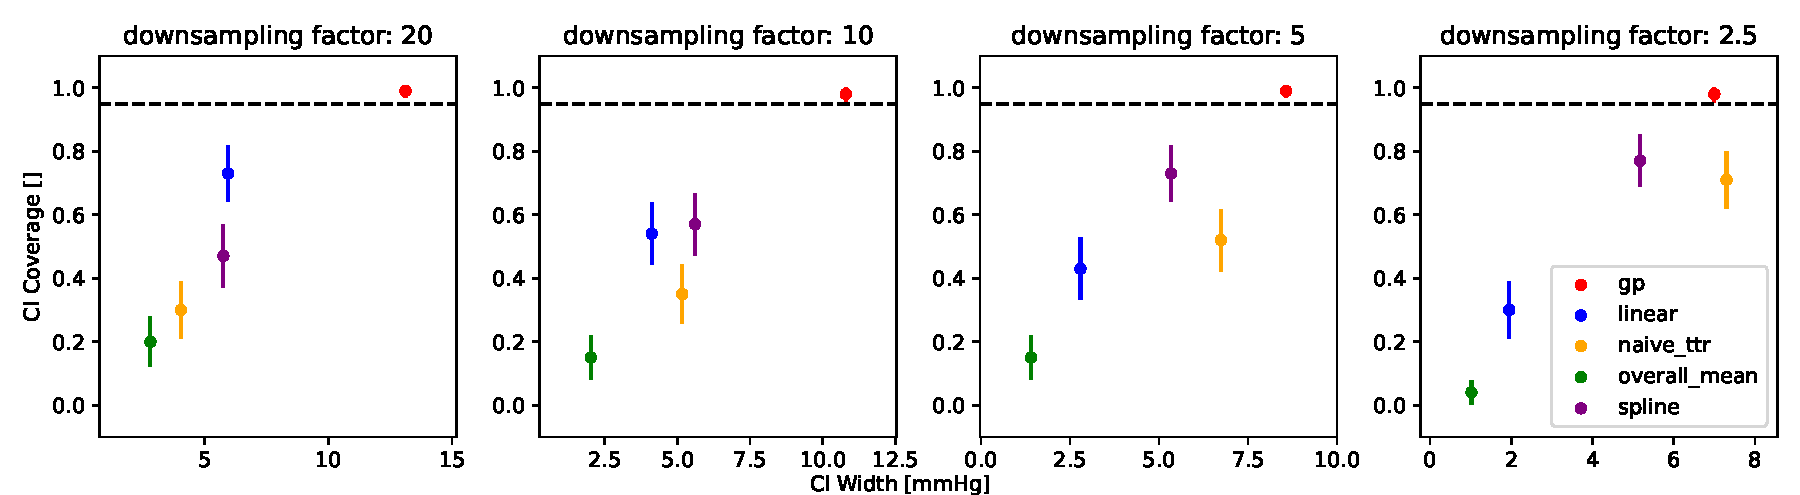
\includegraphics[width=0.8\linewidth]{mean_1h_eval_sin_rbf_seasonal_default}
			\caption{Seasonal Sampling}
	\end{figure}

\end{frame}


\begin{frame}
	\frametitle{Results}
	\framesubtitle{Time in Target Range} % Optional subtitle

	Simulation over a 100 samples from true GP

	\begin{figure}
			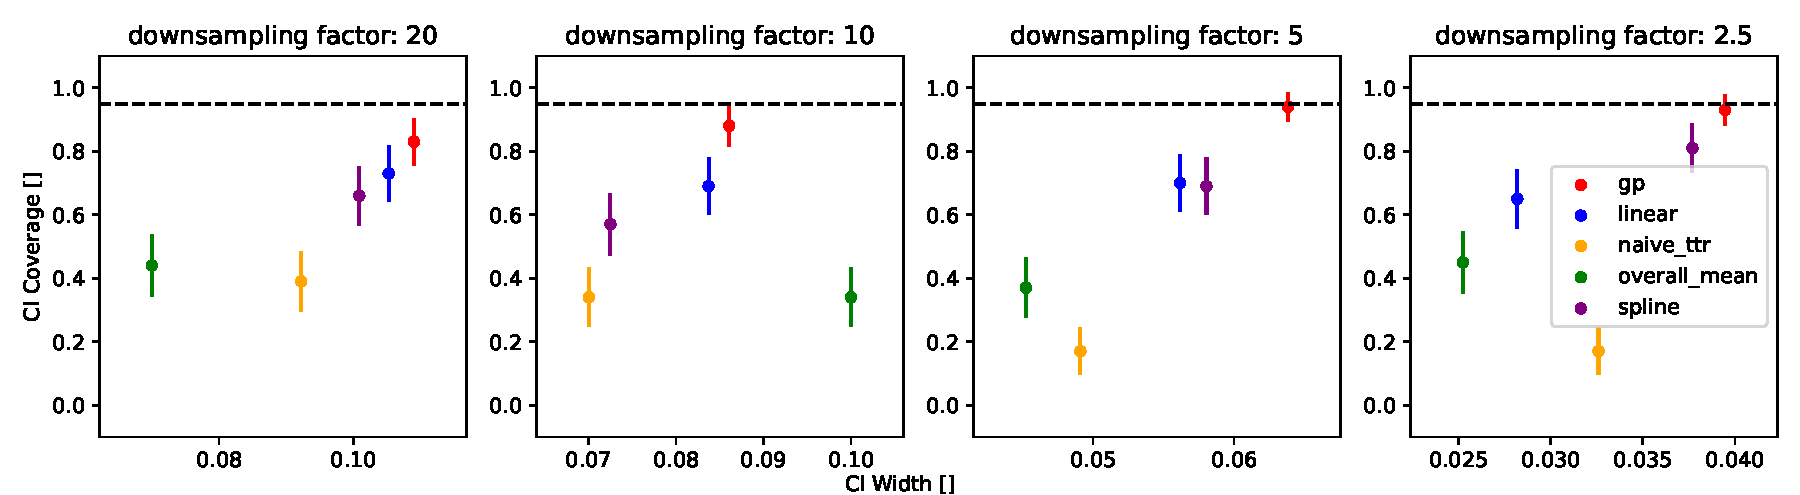
\includegraphics[width=0.85\linewidth]{ttr_eval_sin_rbf_default}
			\caption{Uniform Sampling}
	\end{figure}

	\begin{figure}
			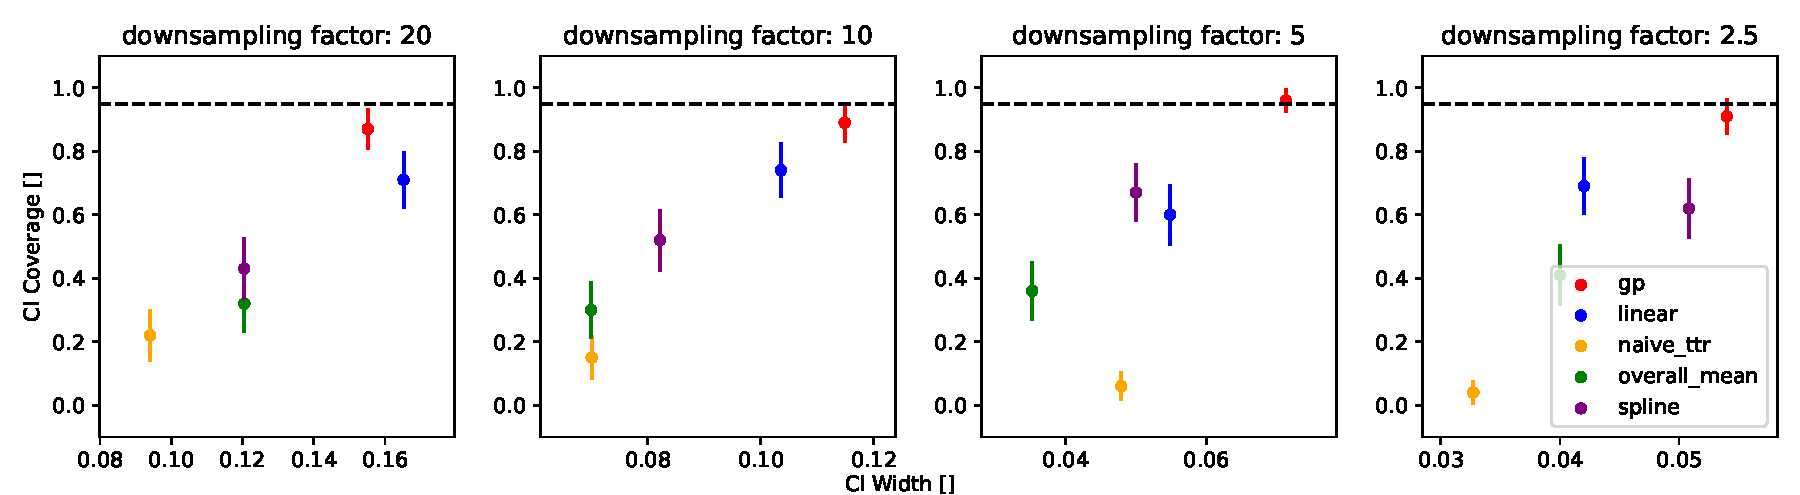
\includegraphics[width=0.85\linewidth]{ttr_eval_sin_rbf_seasonal_default}
			\caption{Seasonal Sampling}
	\end{figure}

\end{frame}


\section{Discussion}

\begin{frame}
	\frametitle{Discussion}

	\begin{table}
	\small
	\centering
	\begin{tabular}{|c|m{3.2cm}|m{3.2cm}|m{3.2cm}|}

  	\hline

  	Method & weekly mean & hourly mean & TTR \\
	\hline

	GP & \cellcolor{green}
	 \begin{itemize}
		 \item underestimates uncertainty
	 \end{itemize}

	& \cellcolor{green}\textbf{Winner}
	&
	\cellcolor{yellow}\textbf{Winner}
	\\
  	\hline

	Linear
	& \cellcolor{green}\textbf{Winner}
%	 \begin{itemize}
%		 \item does not improve much with more data
%	 \end{itemize}
	& \cellcolor{red}
	 \begin{itemize}
		 \item underestimates uncertainty
		 \item does not improve with more data
	 \end{itemize}
	& \cellcolor{red}
	 \begin{itemize}
	 \item does not improve with more data
	 \end{itemize}
	\\
  	\hline

	Spline
	& \cellcolor{green}
	 \begin{itemize}
		 \item very large CI for low data density
	 \end{itemize}
	& \cellcolor{green}
	 \begin{itemize}
		 \item very large CI for low data density
	 \end{itemize}
	& \cellcolor{yellow}
	\begin{itemize}
		\item reasonable CI width also for low data density
	\end{itemize} \\
  	\hline
	\end{tabular}
	\end{table}

\end{frame}



\begin{frame}

	\frametitle{Discussion}


	GP vs Spline vs Linear
	\begin{itemize}
		\item Linear regression performs best if there is very little data
		and a lot of noise.
		Very rigid assumption on the shape of the function.
		(parametric)

		\item Spline regression is more flexible and data dependent.
		It makes no assumption on the periodicity of the function.
		(non parametric)

		\item GP does implicitly model the cyclic pattern by using a cyclic
		kernel function but the shape of the predicted function is very flexible and
		data dependent.
		(non parametric and Bayesian)
	\end{itemize}

	\bigskip

	\begin{itemize}
		\item All methods perform worse with seasonal sampling
		\item Naive overall mean does give reasonable estimates of the weekly
		mean, when there is uniform sampling
		\item Naive TTR is not a good estimator for TTR
		\item GP is very good at predicting the hourly mean and assessing
		local uncertainty
		\item Only GP models the AR component.
		Since AR component it is much smaller
		then the measurement noise (and the cyclic pattern) one can probably
		do without it.
	\end{itemize}

%	\begin{itemize}
%		\item spline huge confidence intervals for very low data frequency
%		\item Linear does not improve with more data. Gives decent weekly mean estimates
%  also for very low data densities and when there is seasonal sampling.
%  Does not estimate the 1h mean and TTR values as well as GP and spline.
%		\item Naive TTR is not a good estimator of TTR.
%	\end{itemize}

%	\begin{itemize}
%		\item Measurement noise variance $\approx 0.5 *$ total variance
%		\item AR(1) component variance $\approx 0.1 *$ measurement noise variance
%		\item Seasonal Component variance $\approx 21 \approx 0.4 *$ total variance (for sinus this equal amplitude of 8. $Var(\sin{x}) = \frac{\text{ampl}^2}{2}$)
%		\item GP can assess local uncertainty due to missing value, which is not needed when evaluating 1 week mean
%		\item Simulation restricted to perfect seasonal patterns
%	\end{itemize}

\end{frame}



\begin{frame}
	\frametitle{Limitations and Potential Next Steps}

	Simulation:
	\begin{itemize}
		\item Cyclic pattern does not evolve over time
		\begin{itemize}
			\item Multiply ExpSineSquare kernel with RBF kernel
		\end{itemize}
		\item Using GPs for simulation might favor GP regression
		\begin{itemize}
			\item Use other simulation method
			\item Add non-Gaussian errors
			\item Use different kernel combination for GP simulation and for
			GP fitting
		\end{itemize}
		\item Measurement error and AR component largely unknown:
		\begin{itemize}
			\item Investigate performance when there is a larger AR component
		\end{itemize}

	\end{itemize}

	\bigskip

	Baseline Method:
	\begin{itemize}
		\item Investigate failure of spline regression for very low data density
	\end{itemize}

\end{frame}




%\begin{frame}
%	\frametitle{Results}
%	\framesubtitle{Weekly Mean} % Optional subtitle
%
%	Simulation over a 100 samples from true GP
%
%	\begin{figure}
%			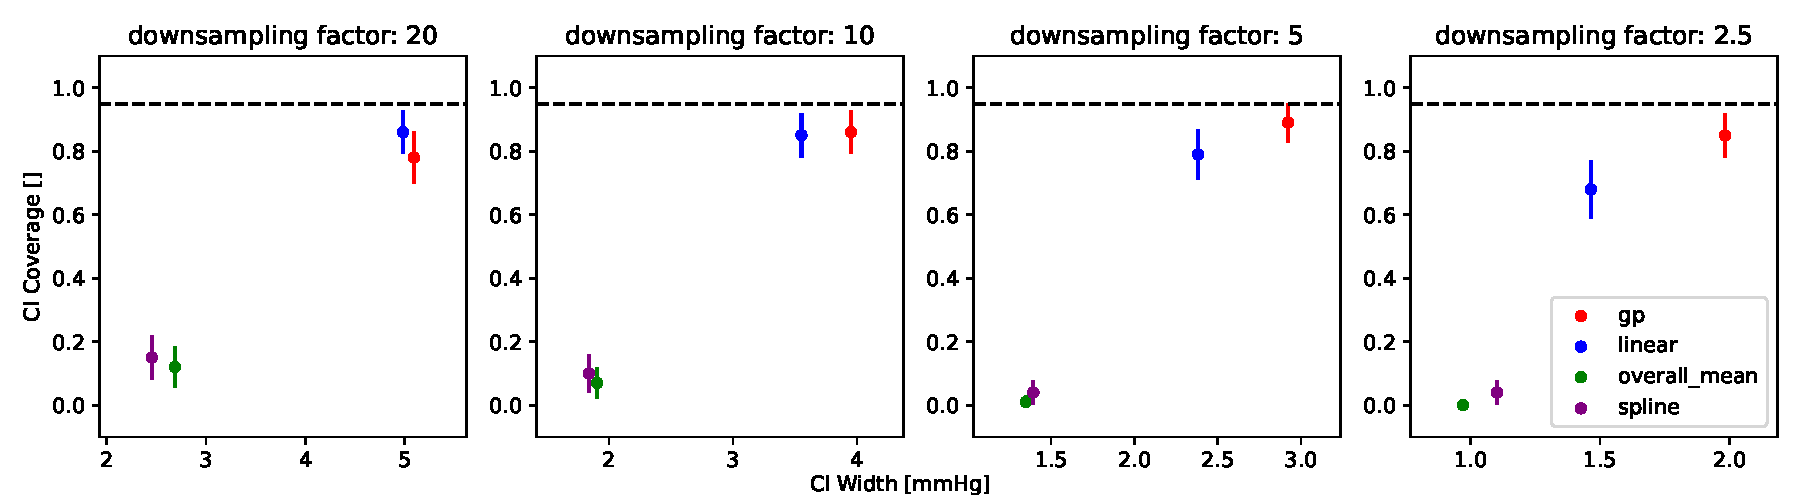
\includegraphics[width=0.8\linewidth]{overall_mean_eval_sin_rbf_seasonal_extreme}
%			\caption{Extreme Seasonal Sampling}
%	\end{figure}
%\end{frame}


%\begin{frame}
%	\frametitle{Outlook - Weekly BP Mean}
%	\begin{figure}
%		\includegraphics[width=0.7\linewidth]{plot_overall_mean_ou_bounded_seasonal_sin_rbf_0.20}
%%			\caption{Periodic Kernel with different length scale}
%	\end{figure}
%
%
%	\begin{table}
%		\begin{tabular}{l l l}
%			\toprule
%			\textbf{metric} & \textbf{GP Predicted Mean} & \textbf{Sample Mean}\\
%			\midrule
%			ci covered & True & False \\
%			predictive probability dens. & 0.25904 & $<$ 0.00001 \\
%			mse & 0.0030 & 4.3988 \\
%			ci width &  0.231 & 0.012 \\
%			\bottomrule
%		\end{tabular}
%%		\caption{}
%
%%		{'ci_overall_mean_lb': -13.305443087675325, 'ci_overall_mean_ub': -13.07422728777426, 'overall_mean_covered': 1, 'ci_overall_width': 0.2312157999010651, 'pred_prob_overall_mean': 0.25903971192446634, 'mse_overll_mean': 0.0030048794026204416, 'covered_fraction_fun': 0.9678571428571429, 'kl_fun': 189561702.44658434, 'pred_logprob': 1182.5772622643588, 'mse': 0.1775464329777053}
%%		{'ci_overall_mean_lb': -11.043858712746218, 'ci_overall_mean_ub': -11.031493422441432, 'overall_mean_covered': 0, 'ci_overall_width': 0.012365290304785503, 'pred_prob_overall_mean': 0.0, 'mse_overll_mean': 4.39884489044144, 'covered_fraction_fun': 0.05476190476190476, 'kl_fun': 11412263.566746384, 'pred_logprob': -720975.0783134875, 'mse': 14.386045805246933}
%
%	\end{table}
%
%
%\end{frame}
%
%
%\begin{frame}
%	\frametitle{Outlook}
%
%	Target measures ?
%	\begin{itemize}
%		\item TTR
%		\item day/night BP (fit trapez model to extracted cyclic pattern, weighting based on cyclic pattern)
%		\item $\dots$
%	\end{itemize}
%
%\end{frame}
%


%\begin{frame}
%	\frametitle{Computational Complexity}
%
%	\begin{itemize}
%		\item update posterior (when new data arrives)
%		\item same user hyperparameters assume to be constant (updated every 2 weeks ?)
%	\end{itemize}
%
%\end{frame}


%%------------------------------------------------
%
%\begin{frame}
%	\frametitle{Lists}
%	\framesubtitle{Bullet Points and Numbered Lists} % Optional subtitle
%
%	\begin{itemize}
%		\item Lorem ipsum dolor sit amet, consectetur adipiscing elit
%		\item Aliquam blandit faucibus nisi, sit amet dapibus enim tempus
%		\begin{itemize}
%			\item Lorem ipsum dolor sit amet, consectetur adipiscing elit
%			\item Nam cursus est eget velit posuere pellentesque
%		\end{itemize}
%		\item Nulla commodo, erat quis gravida posuere, elit lacus lobortis est, quis porttitor odio mauris at libero
%	\end{itemize}
%
%	\bigskip % Vertical whitespace
%
%	\begin{enumerate}
%		\item Nam cursus est eget velit posuere pellentesque
%		\item Vestibulum faucibus velit a augue condimentum quis convallis nulla gravida
%	\end{enumerate}
%\end{frame}
%
%%------------------------------------------------
%
%\subsection{Blocks}
%
%\begin{frame}
%	\frametitle{Blocks of Highlighted Text}
%
%	\begin{block}{Block Title}
%		Lorem ipsum dolor sit amet, consectetur adipiscing elit. Integer lectus nisl, ultricies in feugiat rutrum, porttitor sit amet augue.
%	\end{block}
%
%	\begin{exampleblock}{Example Block Title}
%		Aliquam ut tortor mauris. Sed volutpat ante purus, quis accumsan.
%	\end{exampleblock}
%
%	\begin{alertblock}{Alert Block Title}
%		Pellentesque sed tellus purus. Class aptent taciti sociosqu ad litora torquent per conubia nostra, per inceptos himenaeos.
%	\end{alertblock}
%
%	\begin{block}{} % Block without title
%		Suspendisse tincidunt sagittis gravida. Curabitur condimentum, enim sed venenatis rutrum, ipsum neque consectetur orci.
%	\end{block}
%\end{frame}
%
%%------------------------------------------------
%
%\subsection{Columns}
%
%\begin{frame}
%	\frametitle{Multiple Columns}
%	\framesubtitle{Subtitle} % Optional subtitle
%
%	\begin{columns}[c] % The "c" option specifies centered vertical alignment while the "t" option is used for top vertical alignment
%		\begin{column}{0.45\textwidth} % Left column width
%			\textbf{Heading}
%			\begin{enumerate}
%				\item Statement
%				\item Explanation
%				\item Example
%			\end{enumerate}
%		\end{column}
%		\begin{column}{0.5\textwidth} % Right column width
%			Lorem ipsum dolor sit amet, consectetur adipiscing elit. Integer lectus nisl, ultricies in feugiat rutrum, porttitor sit amet augue. Aliquam ut tortor mauris. Sed volutpat ante purus, quis accumsan dolor.
%		\end{column}
%	\end{columns}
%\end{frame}
%
%%------------------------------------------------
%
%\section{Table and Figure Examples}
%
%\subsection{Table}
%
%\begin{frame}
%	\frametitle{Table}
%	\framesubtitle{Subtitle} % Optional subtitle
%
%	\begin{table}
%		\begin{tabular}{l l l}
%			\toprule
%			\textbf{Treatments} & \textbf{Response 1} & \textbf{Response 2}\\
%			\midrule
%			Treatment 1 & 0.0003262 & 0.562 \\
%			Treatment 2 & 0.0015681 & 0.910 \\
%			Treatment 3 & 0.0009271 & 0.296 \\
%			\bottomrule
%		\end{tabular}
%		\caption{Table caption}
%	\end{table}
%\end{frame}
%
%%------------------------------------------------
%
%%\subsection{Figure}
%%
%%\begin{frame}
%%	\frametitle{Figure}
%%
%%	\begin{figure}
%%		\includegraphics[width=0.8\linewidth]{creodocs_logo.pdf}
%%		\caption{Creodocs logo.}
%%	\end{figure}
%%\end{frame}
%
%%------------------------------------------------
%
%\section{Mathematics}
%
%\begin{frame}
%	\frametitle{Definitions \& Examples}
%
%	\begin{definition}
%		A \alert{prime number} is a number that has exactly two divisors.
%	\end{definition}
%
%	\smallskip % Vertical whitespace
%
%	\begin{example}
%		\begin{itemize}
%			\item 2 is prime (two divisors: 1 and 2).
%			\item 3 is prime (two divisors: 1 and 3).
%			\item 4 is not prime (\alert{three} divisors: 1, 2, and 4).
%		\end{itemize}
%	\end{example}
%
%	\smallskip % Vertical whitespace
%
%	You can also use the \texttt{theorem}, \texttt{lemma}, \texttt{proof} and \texttt{corollary} environments.
%\end{frame}
%
%%------------------------------------------------
%
%\begin{frame}
%	\frametitle{Theorem, Corollary \& Proof}
%
%	\begin{theorem}[Mass--energy equivalence]
%		$E = mc^2$
%	\end{theorem}
%
%	\begin{corollary}
%		$x + y = y + x$
%	\end{corollary}
%
%	\begin{proof}
%		$\omega + \phi = \epsilon$
%	\end{proof}
%\end{frame}
%
%%------------------------------------------------
%
%\begin{frame}
%	\frametitle{Equation}
%
%	\begin{equation}
%		\cos^3 \theta =\frac{1}{4}\cos\theta+\frac{3}{4}\cos 3\theta
%	\end{equation}
%\end{frame}
%
%%------------------------------------------------
%
%\begin{frame}[fragile] % Need to use the fragile option when verbatim is used in the slide
%	\frametitle{Verbatim}
%
%	\begin{example}[Theorem Slide Code]
%		\begin{verbatim}
%			\begin{frame}
%				\frametitle{Theorem}
%				\begin{theorem}[Mass--energy equivalence]
%					$E = mc^2$
%				\end{theorem}
%		\end{frame}\end{verbatim} % Must be on the same line
%	\end{example}
%\end{frame}
%
%%------------------------------------------------
%
%\begin{frame}
%	Slide without title.
%\end{frame}
%
%%------------------------------------------------
%
%\section{Referencing}
%
%\begin{frame}
%	\frametitle{Citing References}
%
%	An example of the \texttt{\textbackslash cite} command to cite within the presentation:
%
%	\bigskip % Vertical whitespace
%
%	This statement requires citation \cite{p1,p2}.
%\end{frame}
%
%%------------------------------------------------
%
%\begin{frame} % Use [allowframebreaks] to allow automatic splitting across slides if the content is too long
%	\frametitle{References}
%
%	\begin{thebibliography}{99} % Beamer does not support BibTeX so references must be inserted manually as below, you may need to use multiple columns and/or reduce the font size further if you have many references
%		\footnotesize % Reduce the font size in the bibliography
%
%		\bibitem[Smith, 2022]{p1}
%			John Smith (2022)
%			\newblock Publication title
%			\newblock \emph{Journal Name} 12(3), 45 -- 678.
%
%		\bibitem[Kennedy, 2023]{p2}
%			Annabelle Kennedy (2023)
%			\newblock Publication title
%			\newblock \emph{Journal Name} 12(3), 45 -- 678.
%	\end{thebibliography}
%\end{frame}
%
%%----------------------------------------------------------------------------------------
%%	ACKNOWLEDGMENTS SLIDE
%%----------------------------------------------------------------------------------------
%
%\begin{frame}
%	\frametitle{Acknowledgements}
%
%	\begin{columns}[t] % The "c" option specifies centered vertical alignment while the "t" option is used for top vertical alignment
%		\begin{column}{0.45\textwidth} % Left column width
%			\textbf{Smith Lab}
%			\begin{itemize}
%				\item Alice Smith
%				\item Devon Brown
%			\end{itemize}
%			\textbf{Cook Lab}
%			\begin{itemize}
%				\item Margaret
%				\item Jennifer
%				\item Yuan
%			\end{itemize}
%		\end{column}
%		\begin{column}{0.5\textwidth} % Right column width
%			\textbf{Funding}
%			\begin{itemize}
%				\item British Royal Navy
%				\item Norwegian Government
%			\end{itemize}
%		\end{column}
%	\end{columns}
%\end{frame}
%
%%%----------------------------------------------------------------------------------------
%%%	CLOSING SLIDE
%%%----------------------------------------------------------------------------------------
%%
%%\begin{frame}[plain] % The optional argument 'plain' hides the headline and footline
%%	\begin{center}
%%		{\Huge The End}
%%
%%		\bigskip\bigskip % Vertical whitespace
%%
%%		{\LARGE Questions? Comments?}
%%	\end{center}
%%\end{frame}
%%
%%%----------------------------------------------------------------------------------------
%%
\end{document}
%%




% data fraction 0.5, amplitude as mean of day and night, measurement noise if doubled ?,
% spline (fix it)


